% Asset ID: AS2MeasuresLocationSpreadTikZ-001
% Source: S1-Chp2-MeasuresOfLocationAndSpread.pdf page 6; transcript section 1
% Related lesson section: Measures of Location and Measures of Spread
% Purpose: Show central tendency as part of location, and spread as a separate family.
\documentclass[tikz,border=8pt]{standalone}
\usepackage{amsmath}
\usetikzlibrary{positioning, shapes.geometric, fit}
\begin{document}
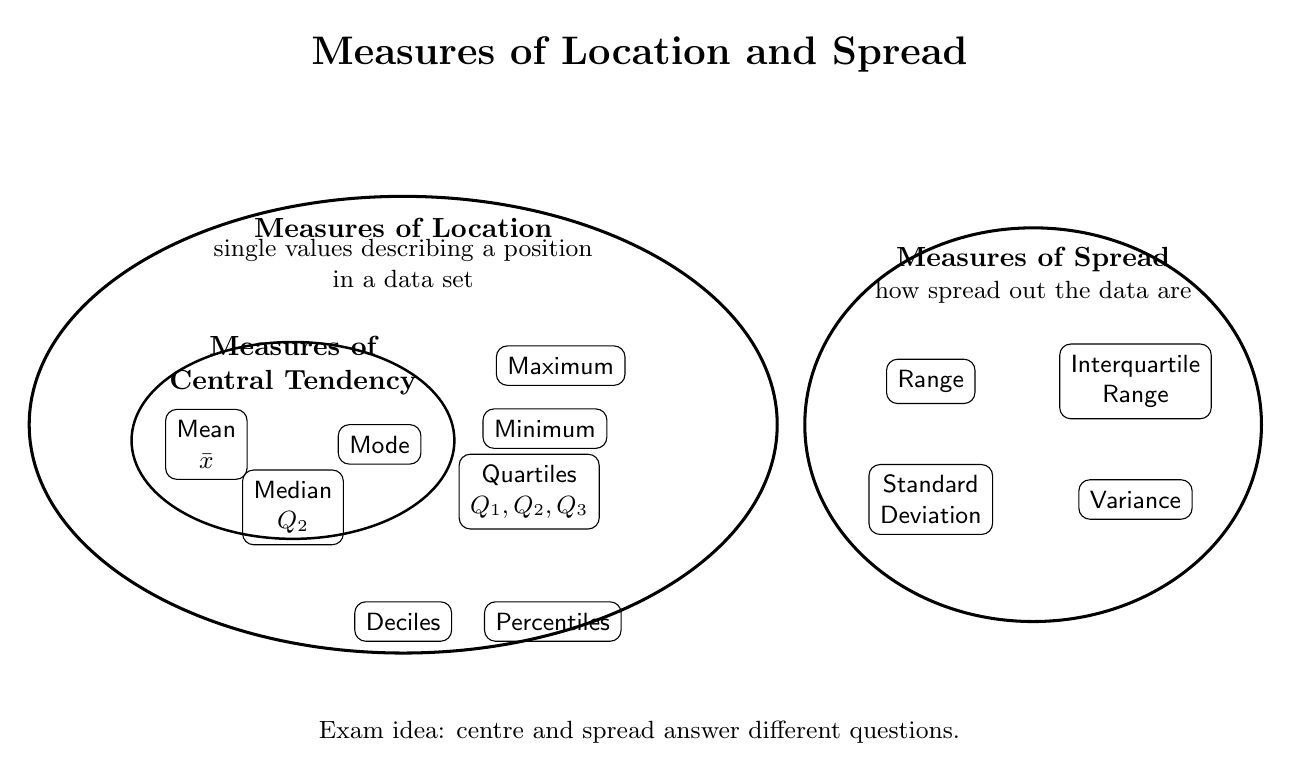
\begin{tikzpicture}[font=\sffamily, box/.style={draw, rounded corners=5pt, align=center, inner sep=6pt}, smallbox/.style={draw, rounded corners=4pt, align=center, inner sep=4pt, font=\small\sffamily}]
\node[font=\Large\bfseries] at (0,5.2) {Measures of Location and Spread};
\node[draw, ellipse, minimum width=9.5cm, minimum height=5.8cm, line width=1.1pt] at (-3,0.5) {};
\node[font=\bfseries, align=center] at (-3,3.0) {Measures of Location};
\node[align=center, font=\small] at (-3,2.55) {single values describing a position\\in a data set};
\node[draw, ellipse, minimum width=4.1cm, minimum height=2.5cm, line width=0.9pt] at (-4.4,0.3) {};
\node[font=\bfseries, align=center] at (-4.4,1.25) {Measures of\\Central Tendency};
\node[smallbox] at (-5.5,0.25) {Mean\\$\bar{x}$};
\node[smallbox] at (-4.4,-0.55) {Median\\$Q_2$};
\node[smallbox] at (-3.3,0.25) {Mode};
\node[smallbox] at (-1.0,1.25) {Maximum};
\node[smallbox] at (-1.2,0.45) {Minimum};
\node[smallbox] at (-1.4,-0.35) {Quartiles\\$Q_1,Q_2,Q_3$};
\node[smallbox] at (-3.0,-2.0) {Deciles};
\node[smallbox] at (-1.1,-2.0) {Percentiles};
\node[draw, ellipse, minimum width=5.8cm, minimum height=5.0cm, line width=1.1pt] at (5.0,0.5) {};
\node[font=\bfseries, align=center] at (5.0,2.6) {Measures of Spread};
\node[align=center, font=\small] at (5.0,2.18) {how spread out the data are};
\node[smallbox] at (3.7,1.05) {Range};
\node[smallbox] at (6.3,1.05) {Interquartile\\Range};
\node[smallbox] at (3.7,-0.45) {Standard\\Deviation};
\node[smallbox] at (6.3,-0.45) {Variance};
\node[align=center, font=\small] at (0,-3.4) {Exam idea: centre and spread answer different questions.};
\end{tikzpicture}
\end{document}
